% Submission template — ICLR 2027.
%
% DOCUMENT CLASS: the official style files were published at
% https://media.iclr.cc/Conferences/ICLR2027/iclr-2027-style-files.zip and are
% vendored in paper/inputs/iclr2027/ (copy in final/ so that directory compiles
% standalone). ICLR 2027 is SINGLE COLUMN: \textwidth 5.5in, \textheight 9in,
% 10pt on 11pt leading, with reviewer line-number rulers in the margins. The
% style file owns the geometry, the type sizes, \maketitle, the abstract, the
% section headings and \parskip — do not restate any of them here.
\documentclass{article}

\usepackage{iclr2027_conference}
\usepackage[T1]{fontenc}
\usepackage[utf8]{inputenc}
\usepackage{newtxtext}
\usepackage{amsmath}
\usepackage{amssymb}
\usepackage{graphicx}
\usepackage{booktabs}
\usepackage{multirow}
\usepackage{caption}
\usepackage[hidelinks]{hyperref}
\usepackage{xcolor}
\usepackage{colortbl}
\usepackage{microtype}
\usepackage{nicefrac}
\usepackage{url}
\usepackage{cleveref}

\captionsetup{labelfont=bf}
\clubpenalty=10000
\widowpenalty=10000
\displaywidowpenalty=10000
\makeatletter\@secpenalty=-3000\makeatother
\setcounter{topnumber}{3}
\setcounter{bottomnumber}{2}
\setcounter{totalnumber}{4}
\renewcommand{\bottomfraction}{0.6}
\renewcommand{\floatpagefraction}{0.7}
\setlength{\textfloatsep}{11pt plus 2pt minus 2pt}
\setlength{\intextsep}{11pt plus 2pt minus 2pt}

\title{What a Language Model Does with a Solver\\
Certificate: An Answer-Evidence Decomposition\\
Across Fourteen Models}
% Anonymous: iclr2027_conference.sty prints the double-blind author block
% itself while \iclrfinalcopy stays commented out. \author is unused there but
% kept so \maketitle has something if the final copy switch is ever flipped.
\author{Anonymous authors\\Paper under double-blind review}
\date{}

\begin{document}
\maketitle

\begin{abstract}
Solver-, tool- and retrieval-augmented systems report large accuracy gains,
routinely read as evidence that the model used the supplied material. Two
mechanisms give the same number: reading a supplied answer, and reasoning over
supplied state. The standard control, a same-shape irrelevant record, separates
neither. We build one that does, holding every surface property we could
enumerate and audit fixed while destroying validity alone, across four sealed
experiments and three robustness checks: $38{,}424$ scored responses,
re-derivable from released receipts. Asked what a model does with a
certificate, the instrument returns a different answer for almost every
checkpoint, arm and inference runtime. The share of the state effect that
survives destroying validity is $98.3\%$ on one checkpoint and $40.4$--$51.4\%$
on another; inference depth is one step on two checkpoints and not on a third;
one model is a usable interface under one inference stack and below the
viability floor under another, on identical weights. One result does not move.
Given a certificate whose fabricated final rule establishes the query's
negation, all three checkpoints answer incorrectly on $189$, $186$ and $192$ of
$192$ items, and the strongest abstains on $0$ of $192$ broken certificates.
Mechanism claims about solver assistance do not transfer between checkpoints.
The failure to check the solver does.
\end{abstract}

\section{Introduction}
% Single column: a [t] float declared here is legal at the top of page 1, which
% puts it ABOVE \maketitle --- the two-column build could not do that because
% the title spans the columns and the column tops start below it. Suppressing
% top floats on this page only leaves the bottom of page 1 as the first legal
% slot, so the pull figure stays on page 1 and stays under the title.
\suppressfloats[t]

\begin{figure}[tb]
\centering

\includegraphics[width=0.82\textwidth]{figures/answer_state_factorial.png}
\caption{\textbf{The instrument.} A solver certificate carries an answer and
the state it follows from, and accuracy adds the two together. Across by whether
the record carries the answer, down by whether it carries the state: every arrow
is then a one-factor edge that attributes. Cells give correct items of 192 for
the reanalysed experiment. The dashed diagonal moves both factors at once, which
is why its null attributed to neither.}
\label{fig:factorial}
\end{figure}

Pairing a language model with an external solver, tool or retrieval index
reliably raises accuracy on tasks the model cannot do alone. Systems that
translate a problem into a formal representation, dispatch it to a symbolic
engine and return the verdict through the model report large end-to-end gains
\citep{pan2023logiclm,olausson2023linc,ye2023satlm,gao2022pal,schick2023toolformer,yang2023leandojo,lewis2020retrievalaugmented}.
Those gains are routinely read as evidence that the model \emph{used} the
supplied material.

That reading is underdetermined. Under \emph{answer reading} the supplied record
contains the conclusion and the model copies it out; under \emph{state use} the
model works with the supplied premises and completes the inference itself. Both
give the same accuracy. The standard control, a same-shape but irrelevant
record, rules out proof length, formatting and generic validity, but not answer
reading: a prefix stopping one step short still names the query's subject and
predicate in adjacent lines, so a model that only checks co-occurrence
reproduces every number a reasoning model would.

The distinction is not academic. A model completing a supplied inference has
some purchase on whether that inference is sound; a model matching surface
co-occurrence has none, and anything built on it inherits the solver's errors in
silence. No accuracy number separates the two.

Separating them needs a control that holds surface form fixed and destroys
validity alone. We build one and apply it across four sealed experiments and three
robustness checks on frozen small models, scoring by direct next-token
likelihood over verified single-token candidates so that no free text is parsed.

\textbf{The instrument works, and almost nothing it returns transfers.}
Breaking validity alone removes $98.3\%$ of the state effect on one checkpoint
and $40.4$--$51.4\%$ on another. Inference depth, order-sensitivity and whether
a model can serve as the interface at all move the same way: they are properties
of a checkpoint, an arm and an inference runtime, not of the architecture. We
therefore offer the method and no general value, ours included. The boundary is
strict, too: on the Qwen checkpoints every arm without a near-complete chain
returns $d' = 0$, so high accuracy with a full certificate describes a faithful
transcriber rather than a reasoner.

\textbf{One result does not move.} Given a certificate whose fabricated final
rule establishes the query's negation, all three checkpoints answer incorrectly
on $189$, $186$ and $192$ of $192$ items, and none abstains on a broken one.
Mechanism claims about solver assistance do not transfer between checkpoints.
The failure to check the solver does.

What is new is the instrument: a $2\times2$ separating solver-supplied answers
from solver-supplied state (\cref{fig:factorial}), a surface-matched invalid
certificate certified per item, and a closure certifier for queries nothing
decides. We apply it to fourteen models
\citep{team2024qwen,grattafiori2024llama,team2025gemma,microsoft2025phi,team2024olmo,allal2025smollm}.

\section{Related Work}

Chain-of-thought made intermediate steps part of the output
\citep{wei2022chainofthought}, and a literature then asked whether the answer
rests on them: explanations omit the biasing features that drive the prediction
\citep{turpin2023language}, injected mistakes are often ignored
\citep{lanham2023measuring,arcuschin2025chainofthought}, answer-determining
hints go unverbalised \citep{chen2025reasoning}, and one response is to make the
trace a program a solver executes \citep{lyu2023faithful}. Neurosymbolic work
puts the formal step outside the model altogether
\citep{pan2023logiclm,olausson2023linc,ye2023satlm,gao2022pal}, and the pattern
extends to tool use \citep{schick2023toolformer}, premise selection
\citep{yang2023leandojo} and retrieval \citep{lewis2020retrievalaugmented}.

Both leave our question open. The first intervenes on \emph{model-generated}
traces, where ignoring a mistake is unfaithful; ours is externally supplied,
formally verified state, where following a corrupted one is unsafe. The second
reports end-to-end accuracy, which cannot separate the solver's \emph{answer}
from its \emph{state} and assumes the solver correct, though the model side is
not neutral to context \citep{shi2023large,xie2023adaptive}.

The task family descends from rule-based deductive datasets in natural language
\citep{clark2020transformers,tafjord2020proofwriter,saparov2022language,han2022folio}.
Order effects there are large \citep{chen2024premise}, the sets predate the
models evaluated on them \citep{deng2024investigating,golchin2023time}, and
counterfactual variants show how much apparent competence rests on familiarity
\citep{wu2023reasoning}. None supplies the matched adversarial certificates an
attribution question needs, so we generate items after model release with
per-item invented vocabularies and build the certificates ourselves.

Prompted classification is biased rather than merely noisy: accuracy swings with
format and example order \citep{zhao2021calibrate}, option order alone moves it
\citep{pezeshkpour2023large,zheng2023large}, likelihood scoring lets strings
compete for probability mass independently of correctness
\citep{holtzman2021surface}, and abstention is its own capability
\citep{kadavath2022language,yin2023large}. On a balanced panel a degenerate
single-label responder is indistinguishable from a chance-level competent one,
so we report $d'$ and criterion $c$ for every arm
\citep{macmillan1991detection,stanislaw1999calculation} with the exact McNemar
test \citep{mcnemar1947note} and bootstrap intervals \citep{efron1987better}.
Two cases here motivate that rather than illustrate it: an arm scoring $50.0\%$
with $d' = 0.00$, and a prespecified criterion of our own passed by models
answering one label almost everywhere.

\section{Method}

\subsection{The answer-evidence decomposition}

A solver certificate carries an answer and the state it follows from, and
\cref{fig:factorial} separates them. \textsc{irrelevant} supplies a valid
derivation for a different entity,
\textsc{conclusion\_only} the derived terminal literal alone,
\textsc{proof\_prefix} the chain with that literal withheld, and \textsc{full}
both, with a no-material baseline outside the square. The experiment we
reanalyse chose the diagonal as its primary contrast.

\begin{table}[tb]
\centering\footnotesize
\caption{\textbf{What the model sees}, from sealed item \texttt{b15-4ef53c71}.
Every prompt is the same 18-line theory in invented vocabulary, then one solver
record, then the query. Only the record changes between arms. Left: the
\textsc{full} record, a complete four-step derivation. Right: what each other
arm does to it. \textsc{broken\_chain} is the word-matching test: line 6 becomes
a different \emph{real} rule of the theory, one that does not fire, so the chain
no longer reaches the query while every surface cue of \textsc{truncate\_1}
survives. \textsc{misleading} instead invents a rule the theory does not
contain.}
\label{tab:stimulus}
\begin{minipage}[t]{0.40\textwidth}
\vspace{0pt}
\ttfamily\scriptsize
\textrm{\textbf{Query:}} Bimol is vrinpek. \textrm{(true)}\\[3pt]
\textrm{\textbf{\textsc{full} record}}\\
1\ \ Bimol is vrasler.\\
2\ \ All vrasler people are deinmal.\\
3\ \ Bimol is deinmal.\\
4\ \ All deinmal people are kuthbror.\\
5\ \ Bimol is kuthbror.\\
6\ \ All kuthbror people are gasplaek.\\
7\ \ Bimol is gasplaek.\\
8\ \ All gasplaek people are vrinpek.\\
9\ \ Bimol is vrinpek.
\end{minipage}\hfill
\begin{minipage}[t]{0.58\textwidth}
\vspace{0pt}
\scriptsize
\begin{tabular}{@{}ll@{}}
\toprule
Arm & Record supplied \\
\midrule
\textsc{none}        & no record at all \\
\textsc{irrelevant}  & same shape, a different entity throughout \\
\textsc{same\_entity\_irrel.} & same entity, an unrelated predicate \\
\textsc{truncate\_1} & lines 1--8: the answer line withheld \\
\textsc{truncate\_2} & lines 1--6: two steps withheld \\
\textsc{truncate\_3} & lines 1--4: three steps withheld \\
\textsc{shuffled}    & lines 1--8 in seeded random order \\
\textsc{broken\_chain} & lines 1--8, but 6 becomes \texttt{All foskdem} \\
                     & \texttt{people are zuftbas.} and 7 becomes \\
                     & \texttt{Bimol is zuftbas.} Line 8 unchanged \\
\textsc{misleading}  & lines 1--9, but 8 becomes \texttt{All gasplaek} \\
                     & \texttt{people are not vrinpek.} and 9 becomes \\
                     & \texttt{Bimol is not vrinpek.} \\
\textsc{full}        & lines 1--9 \\
\bottomrule
\end{tabular}
\end{minipage}
\end{table}

% tab:stimulus is declared here, inside 3.1, rather than beside the 3.2 text
% that cites it, so that it lands on the same page as, or before, its first
% reference. In two columns it was a table* and could only reach a page top;
% single column it can also reach a page bottom, so the placement is far less
% brittle --- but the declaration point still decides which page it competes
% for, and this one is measured.
\textbf{Why the usual control is not enough.} Take a theory in which Kexil is dovrant,
every dovrant thing is plesh, and every plesh thing is marn, with the query
\emph{is Kexil marn?} The standard control gives a same-shape derivation about a
different entity, fixing length, format and generic validity. But the arm it is
compared against ends on \emph{Kexil is plesh}, one line from a rule naming
\emph{marn}: the query's subject and predicate sit in adjacent lines. A model
that never takes the last step, and only registers that the two terms co-occur
where a derivation is heading, reproduces every number a model completing it
would. The square localises the gain to state; it cannot show the state was used
as inference.

\subsection{Surface-matched invalidity: the word-matching test}
\label{sec:broken}
\Cref{tab:stimulus} shows one sealed item and every record we supply for it.
Call the prefix that stops one step short \textsc{truncate\_1}: it is the
strongest arm that withholds the answer, and the one a surface-matching model
can still exploit. \textsc{broken\_chain} strips that exploit. We cut one
intermediate link, so the displayed lines no longer reach the query, holding
fixed against \textsc{truncate\_1} the query-entity occurrence count (audited
per item), the query predicate in the final rule, the line count and the
fact/rule/literal sequence. Every rule displayed is real; exactly one derived
literal is false; all $192$ items are certified to leave the query undecided
under the displayed lines. That gives
\[
\text{total state} = \textsc{truncate\_1} - \textsc{irrelevant},\quad
\text{surface} = \textsc{broken\_chain} - \textsc{irrelevant},
\]
\[
\text{validity} = \textsc{truncate\_1} - \textsc{broken\_chain}.
\]
Five companion arms separate the rest, listed in \cref{tab:stimulus}:
\textsc{same\_entity\_irrelevant} isolates entity repetition, \textsc{shuffled}
isolates line order, and \textsc{truncate\_2} and \textsc{truncate\_3} give a
depth ladder. \textsc{misleading} is the corrupted-solver arm: one fabricated
final rule, absent from the theory, establishes the query's negation, so
following the supplied record means answering incorrectly while the true answer
is unchanged.

\subsection{Certifying that nothing decides a query}

Showing a query is derivable is easy: exhibit the proof. Showing nothing decides
it needs the theory's forward closure saturated. Our certifier works under
open-world semantics with explicit negation, so a negative literal holds only if
something derives it, never by failure to prove the positive. It agrees with a
public corpus \citep{tafjord2020proofwriter} on $23{,}240$ of $23{,}240$
questions, $10{,}440$ of them undecided; passes nine adversarial theories
probing cycles, round-cap overruns, derived negation and absent symbols; and
agrees with an independently written reference on $192$ of $192$ items. No item
enters a sealed panel uncertified.

\section{Experimental Setup}

Every experiment asks a rule-chaining query over a small theory of facts and
universally quantified rules. \Cref{tab:panels} names the seven and says what each
one does.

\begin{table}[tb]
\centering\small
\caption{\textbf{The four experiments and three robustness checks.} Sealed panels
use per-item invented vocabularies, are mutually disjoint, and fix derivation
depth at four. The public corpus validates the certifier only: no item from it
is scored by any model here.}
\label{tab:panels}
\footnotesize
\begin{tabular}{@{}l@{\hskip 1em}l@{\hskip 1em}l@{\hskip 1em}l@{}}
\toprule
Panel & Items & Experiment & What it does \\
\midrule
\texttt{b14} & 192 binary & reanalysis & re-reads a five-arm factorial as the $2\times2$ (\cref{fig:factorial}) \\
\texttt{b15} & 192 binary & validity control & ten matched arms (\cref{tab:stimulus}) on three checkpoints \\
\texttt{b16} & 192 three-class & model sweep & ten models $\times$ five arms, with an \texttt{Unknown} class \\
\texttt{b17}, \texttt{b17b} & \texttt{b15} items & abstention rescoring & re-scores broken certificates, \texttt{Unknown} allowed \\
\midrule
\texttt{b18} & \texttt{b15} items & line-order check & eight permutations of each record \\
\texttt{b16} on CUDA & as \texttt{b16} & runtime check & \texttt{transformers}, not \texttt{mlx-lm}; two larger models \\
\texttt{b15} at scale & \texttt{b15} items & scale check & the same arms at 32.8B and 70.6B \\
\midrule
ProofWriter OWA & 23{,}240 & \multicolumn{2}{l}{certifier validation only \citep{tafjord2020proofwriter}} \\
\bottomrule
\end{tabular}
\end{table}

The abstention rescoring generates no panel. It rescores the validity
control's items with a third candidate available, changing only the instruction line and the candidate set on
byte-identical inputs, and its \textsc{none} arm fixes the abstention floor
under that same instruction. On the sweep's $64$ undecidable items there is
no terminal literal to supply, so those two cells instantiate the $2\times2$
less exactly than the rest. The three robustness checks reuse these
panels: eight line permutations of each certificate, recording where the final
rule and its premise land; the sweep rescored through \texttt{transformers} on
CUDA, adding Llama-3.1-8B and Qwen2.5-14B; and the validity control's own items
on that same stack at Qwen3-32B and Llama-3.3-70B, on rented H100s.

Responses are scored by direct next-token likelihood over verified single-token
candidates: \texttt{Yes}/\texttt{No} for the first two,
\texttt{Yes}/\texttt{No}/\texttt{Unknown} for the others. The model generates no
free text, so no verdict is inferred from prose. Every prompt is instruction,
theory, solver record and query, and the theory is visible in every arm. In the
reanalysis the record's header differs between arms as well as its content, a
confound on that experiment's primary contrast, removed everywhere after it.

\textbf{Models.} The reanalysis and the validity control use one frozen 3B
instruction-tuned checkpoint at 4-bit precision \citep{team2024qwen}, pinned to
byte-identical weights. The sweep scores ten instruction-tuned models from
$0.5$B to $7.6$B across six families
\citep{team2024qwen,grattafiori2024llama,team2025gemma,microsoft2025phi,team2024olmo,allal2025smollm}
through \texttt{mlx-lm}, from pinned mirrors; the runner recorded no dtype,
so we claim no uniform precision across the ten. No gate blocks that run:
delivery is the capability under test, so a model that cannot emit a verdict
reliably is a finding, not an exclusion.

\textbf{Sensitivity, not accuracy.} Accuracy on a balanced panel is
uninterpretable when the responder is biased: one arm below scores $50.0\%$
while discriminating nothing at all. We therefore report $d'$ and criterion $c$
for every arm
\citep{macmillan1991detection,stanislaw1999calculation} using the loglinear
correction, balanced accuracy for the three-class panel (chance $33.3\%$), the
exact two-sided McNemar test \citep{mcnemar1947note} as the decision criterion,
and seeded paired bootstrap intervals \citep{efron1987better} adjusted for
multiple comparisons within declared families.

\section{Results}

\subsection{The state effect is real, and it is validity}

The reanalysis begins from a null: its prespecified primary contrast,
$\textsc{proof\_prefix} - \textsc{conclusion\_only} = -4.7$pp (exact McNemar
$p = 0.078$), was reported as no effect. That contrast is the diagonal. The
edges tell a different story: both channels carry real effect, and not
additively. The state
main effect is $+22.4$pp, the answer main effect $+27.1$pp, and the interaction
$-29.2$pp, larger than either. All four edges of \cref{fig:factorial} clear
exact McNemar $p < 10^{-4}$; the original reported the two state edges as
secondary and neither answer edge at all. This reading is post hoc, re-derived
from the 960 raw receipts by a script that asserts it reproduces all five
published per-arm counts before reporting. The
design is ceiling-limited, \textsc{full} reaching $191/192$, so both
``other factor present'' edges are compressed and the averaged main effects
deflated with them.

The baseline description was also wrong. The model answers \texttt{No}
to $88\%$ of items, and \textsc{irrelevant} returns an identical $9/96$ ``Yes''
rate in both classes at $d' = 0.00$ (\cref{tab:sdt}), below a trivial
always-\texttt{No} strategy's $96/192$.

\begin{table}[tb]
\centering\small
\caption{Signal detection for the reanalysis; hits and false alarms out of 96
each. Apparent chance and zero
sensitivity are not the same thing.}
\label{tab:sdt}
\begin{tabular}{lrrrr}
\toprule
Arm & Hits & FA & $d'$ & $c$ \\
\midrule
\textsc{none} & 9 & 14 & $-0.25$ & $+1.17$ \\
\textsc{irrelevant}      &  9 &  9 & $\mathbf{0.00}$ & $+1.29$ \\
\textsc{conclusion\_only}& 80 &  0 & $+3.52$ & $+0.81$ \\
\textsc{proof\_prefix}   & 71 &  0 & $+3.20$ & $+0.97$ \\
\textsc{full}            & 95 &  0 & $+4.72$ & $+0.20$ \\
\bottomrule
\end{tabular}
\end{table}

Destroying validity alone removes almost all of the state effect.
$\textsc{truncate\_1} - \textsc{broken\_chain} = +60.4$pp (exact McNemar
$p = 6.9\times10^{-18}$, BCa $[+49.0, +68.8]$, entailed subset $n = 96$ as
declared before the run), with $d'$ dropping $2.446$: a change in discrimination,
not in criterion. The total state effect of $+61.5$pp is therefore $+1.0$pp of
surface overlap ($p = 1$) and $+60.4$pp of validity --- a \textbf{validity share
of $98.3\%$}, 95\% percentile $[94.4, 100.0]$ (\cref{tab:arms}).

Two supporting contrasts. Entity repetition explains nothing ($+0.0$pp,
$p = 1$) despite one arm naming the query subject four times and the other not
at all. And depth is a cliff, not a slope, on the Qwen checkpoints: withholding
two steps scores identically to supplying no certificate, $0/96$. Gemma-3-4B is
not in that position, and there the direction is worse than null --- $4/96$
against $22/96$ unaided.

\begin{table}[tb]
\centering\small
\caption{The validity control: ten matched arms scored on three checkpoints, entailed
subset (correct of 96, with signed $d'$). Only the solver record differs between
arms. The share rows give the validity component as a fraction of the total state
effect, against the \textsc{irrelevant} control and against the unaided
\textsc{none} arm; the two coincide wherever unaided competence is zero.}
\label{tab:arms}
\begin{tabular}{lrrrrrr}
\toprule
& \multicolumn{2}{c}{Qwen2.5-3B 4-bit} & \multicolumn{2}{c}{Qwen2.5-3B bf16}
& \multicolumn{2}{c}{Gemma-3-4B} \\
\cmidrule(lr){2-3}\cmidrule(lr){4-5}\cmidrule(lr){6-7}
Arm & /96 & $d'$ & /96 & $d'$ & /96 & $d'$ \\
\midrule
\textsc{none}                    &  0 & $0.00$ &  0 & $0.00$ & \textbf{22} & $1.83$ \\
\textsc{irrelevant}              &  0 & $0.00$ &  0 & $0.00$ &  2 & $0.62$ \\
\textsc{same\_entity\_irrelevant}&  0 & $0.00$ &  0 & $0.00$ &  3 & $0.77$ \\
\textsc{truncate\_3}             &  0 & $0.00$ &  0 & $0.00$ &  4 & $0.88$ \\
\textsc{truncate\_2}             &  0 & $0.00$ &  0 & $0.00$ &  4 & $0.88$ \\
\textsc{truncate\_1}             & 59 & $2.85$ & 72 & $3.23$ & 96 & $5.13$ \\
\textsc{broken\_chain}           &  1 & $0.41$ &  1 & $0.41$ & \textbf{58} & $2.83$ \\
\textsc{shuffled}                & 14 & $1.53$ & 12 & $1.43$ & \textbf{86} & $3.80$ \\
\textsc{misleading}              &  0 & $-4.36$ &  0 & $-4.06$ &  0 & $-5.13$ \\
\textsc{full}                    & 96 & $5.13$ & 96 & $5.13$ & 96 & $5.13$ \\
\midrule
Validity share vs \textsc{irrelevant} & \multicolumn{2}{c}{$98.3\%$}
 & \multicolumn{2}{c}{$98.6\%$} & \multicolumn{2}{c}{$\mathbf{40.4\%}$} \\
Validity share vs \textsc{none}       & \multicolumn{2}{c}{$98.3\%$}
 & \multicolumn{2}{c}{$98.6\%$} & \multicolumn{2}{c}{$\mathbf{51.4\%}$} \\
\bottomrule
\end{tabular}
\end{table}

\subsection{Almost nothing the instrument returns transfers}

\textbf{The instrument transfers; the number it returns does not.} The
decomposition was run on two further checkpoints: the same model at bfloat16,
which isolates quantisation from model identity, and a different family.
\Cref{fig:replication} plots the split.

Quantisation is the smaller effect and leaves the share unchanged. Model
identity is not like that. Gemma-3-4B answers \textsc{broken\_chain} correctly
on $58$ of $96$ items where the other two manage $1$, so the control that
isolates inference on one checkpoint exposes surface exploitation on another.
Its share is $40.4\%$ against the \textsc{irrelevant} control and $51.4\%$
against what it manages unaided; the divergence is the finding, not either
number. The control is not inert on such a model either, costing Gemma most of
its own competence, so any effect measured against it there is inflated. Nor
does order-sensitivity replicate alongside the share (\cref{tab:arms}).

\begin{figure}[tb]
\centering

\includegraphics[width=1.0\textwidth]{figures/validity_share_replication.png}
\caption{The surface and validity components on three checkpoints. Bars give
the decomposition against the \textsc{irrelevant} control; the annotation gives
the share against that control and against what the model manages unaided. The
two denominators coincide on the Qwen checkpoints, which score $0/96$ with no
certificate, and diverge only where a model has competence of its own.}
\label{fig:replication}
\end{figure}

The square itself is no steadier. Across ten models, post hoc from receipts
already collected, the mean state main effect is $+8.7$pp against a mean answer
main effect of $+21.6$pp: the answer channel dominates, and the reanalysis's
$+22.4$pp is not typical. Excluding four responders degenerate in every arm
gives $+14.7$pp against $+28.5$pp; the ordering survives either subset.

Whether a model can serve as the interface at all varies the same way. We had
declared that a model relays non-determination at $\geq 80\%$ recall on
undecidable items with full solver material. Eight of ten passed and the
criterion was invalid: single-class recall is maximised by answering
\texttt{Unknown} to everything, which four models approach. We replace it
\textbf{post hoc} with a floor on every class, minimum per-class recall
$\geq 0.50$, keeping both verdicts in the released results. A second
prespecified criterion, a paired $\textsc{full} - \textsc{none}$ of $20$pp on
those items, is met by five of ten under Holm --- two of them rejected by the
replacement floor, the same gameability by another route
(\cref{tab:models}).

\begin{table}[tb]
\centering\small
\caption{All five arms, all twelve models. Each cell is balanced accuracy
(\%, chance $=33.3$) $/$ minimum per-class recall; bold clears the $0.50$ recall
floor, so \textsc{viable in} is derivable from the cells beside it. Shaded rows
are the scale extension on a second runtime: the parameter
ladder continues, the numbers are not comparable across the rule. Viability is
reported per arm, not per model.}
\label{tab:models}
\begin{tabular}{@{}lrccccc@{\hskip 0.9em}l@{}}
\toprule
Model & B & \textsc{none} & \textsc{irrel} & \textsc{concl} & \textsc{prefix} & \textsc{full} & \textsc{viable in} \\
\midrule
Qwen2.5-0.5B &  0.5 & 35.4/0.00 & 34.9/0.00 & 41.1/0.00 & 43.2/0.00 & 63.5/0.00 & --- \\
OLMo-2-1B    &  1.0 & 35.9/0.00 & 33.3/0.00 & 53.6/0.00 & 34.9/0.00 & 42.2/0.00 & --- \\
Llama-3.2-1B &  1.2 & 33.9/0.00 & 33.9/0.00 & 57.8/0.00 & 36.5/0.00 & 37.0/0.00 & --- \\
Qwen2.5-1.5B &  1.5 & 33.3/0.00 & 33.3/0.00 & 43.2/0.00 & 34.9/0.00 & 37.0/0.00 & --- \\
SmolLM2-1.7B &  1.7 & 33.3/0.00 & 33.3/0.00 & 45.3/0.00 & 39.6/0.00 & 69.3/0.38 & --- \\
Qwen2.5-3B   &  3.0 & 41.1/0.00 & 39.1/0.00 & \textbf{96.4/0.91} & \textbf{74.0/0.56} & \textbf{90.6/0.72} & concl, prefix, full \\
Llama-3.2-3B &  3.2 & 45.8/0.00 & 43.2/0.02 & 67.2/0.02 & 55.2/0.02 & 80.7/0.42 & --- \\
Phi-4-mini   &  3.8 & 44.8/0.00 & 39.6/0.00 & 68.2/0.05 & 71.9/0.33 & \textbf{90.6/0.72} & full \\
Gemma-3-4B   &  4.3 & 63.5/0.36 & 51.0/0.06 & \textbf{100.0/1.00} & \textbf{84.4/0.53} & \textbf{96.4/0.89} & concl, prefix, full \\
Qwen2.5-7B   &  7.6 & 33.3/0.00 & 33.3/0.00 & \textbf{97.9/0.94} & 67.2/0.02 & 71.4/0.14 & \textbf{concl only} \\
\midrule
\rowcolor{black!7} Llama-3.1-8B &  8.0 & 38.5/0.00 & 34.4/0.00 & 65.6/0.00 & 64.6/0.00 & 66.7/0.00 & --- \\
\rowcolor{black!7} Qwen2.5-14B  & 14.7 & 57.3/0.00 & 35.4/0.00 & 80.7/0.42 & 70.3/0.12 & 82.8/0.48 & --- \\
\bottomrule
\end{tabular}
\end{table}

Read by row, that verdict is a property of (model $\times$ arm $\times$ runtime).
Qwen2.5-7B falls from second best in the sweep under
\textsc{conclusion\_only} to $0.141$ minimum per-class recall under
\textsc{full}: supplying the proof state is what breaks it, and it breaks three
of ten models here. Nothing below $3$B clears the floor in any arm, but that is a
floor for \emph{tolerating full certificates} rather than a size law:
Llama-3.1-8B is degenerate in every arm, and Qwen2.5-14B never clears it.

The third factor is the inference stack. Re-scoring the same sealed panel, same
weights, same prompt bytes through \texttt{transformers} on CUDA covers nine of
the ten; eight agree on $95.5$--$99.7\%$ of individual responses with no verdict
moving. Phi-4-mini agrees on $87.9\%$, and its \textsc{full} arm is viable under
one stack and not the other: minimum per-class recall $0.719$ against $0.219$,
on identical weights, flips reaching $3.0$ logits. Gemma-3-4B, which carries the
$40.4$--$51.4\%$ share, is the one model this check cannot cover, so that share
has no runtime replication.

\begin{figure}[tb]
\centering
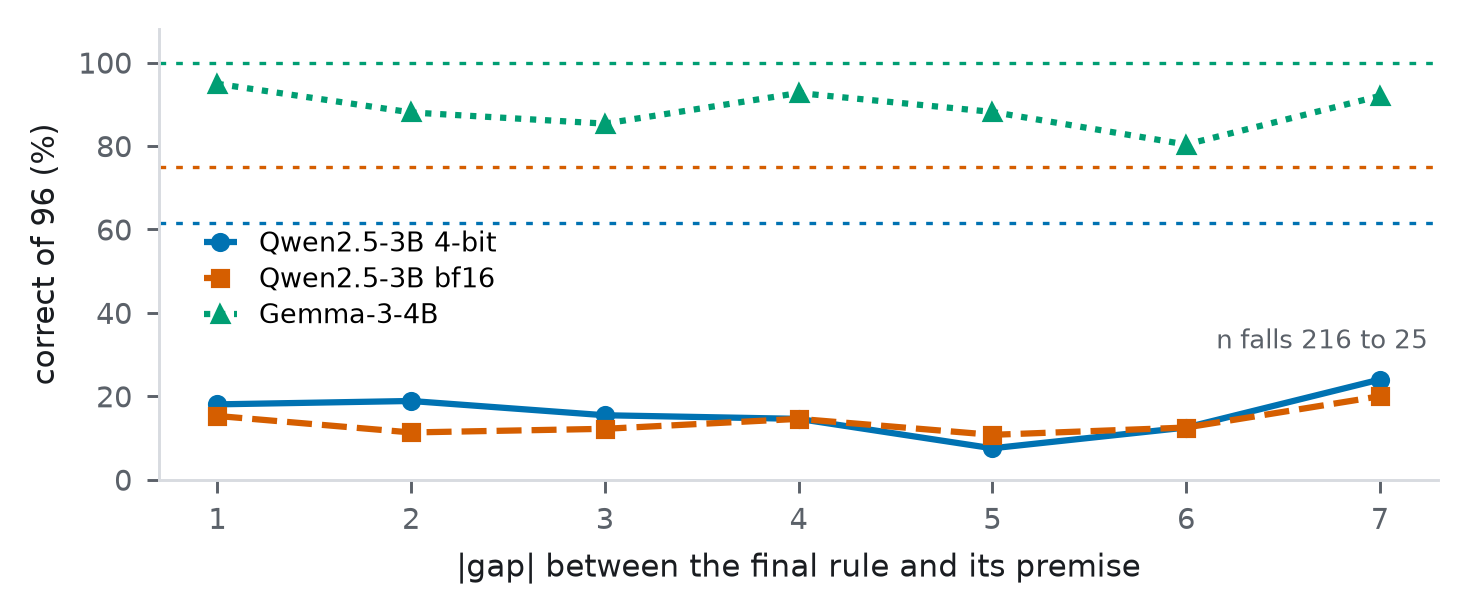
\includegraphics[width=1.0\textwidth]{figures/order_profile.png}
\caption{Accuracy against the gap between the final rule and the premise it
fires on: all seven gaps, all three checkpoints, each checkpoint's
canonical-order score dashed. Distance is flat; direction is not, and the size
of the direction effect is not shared.}
\label{fig:order}
\end{figure}

\subsection{What does not vary}

\begin{figure}[tb]
\centering
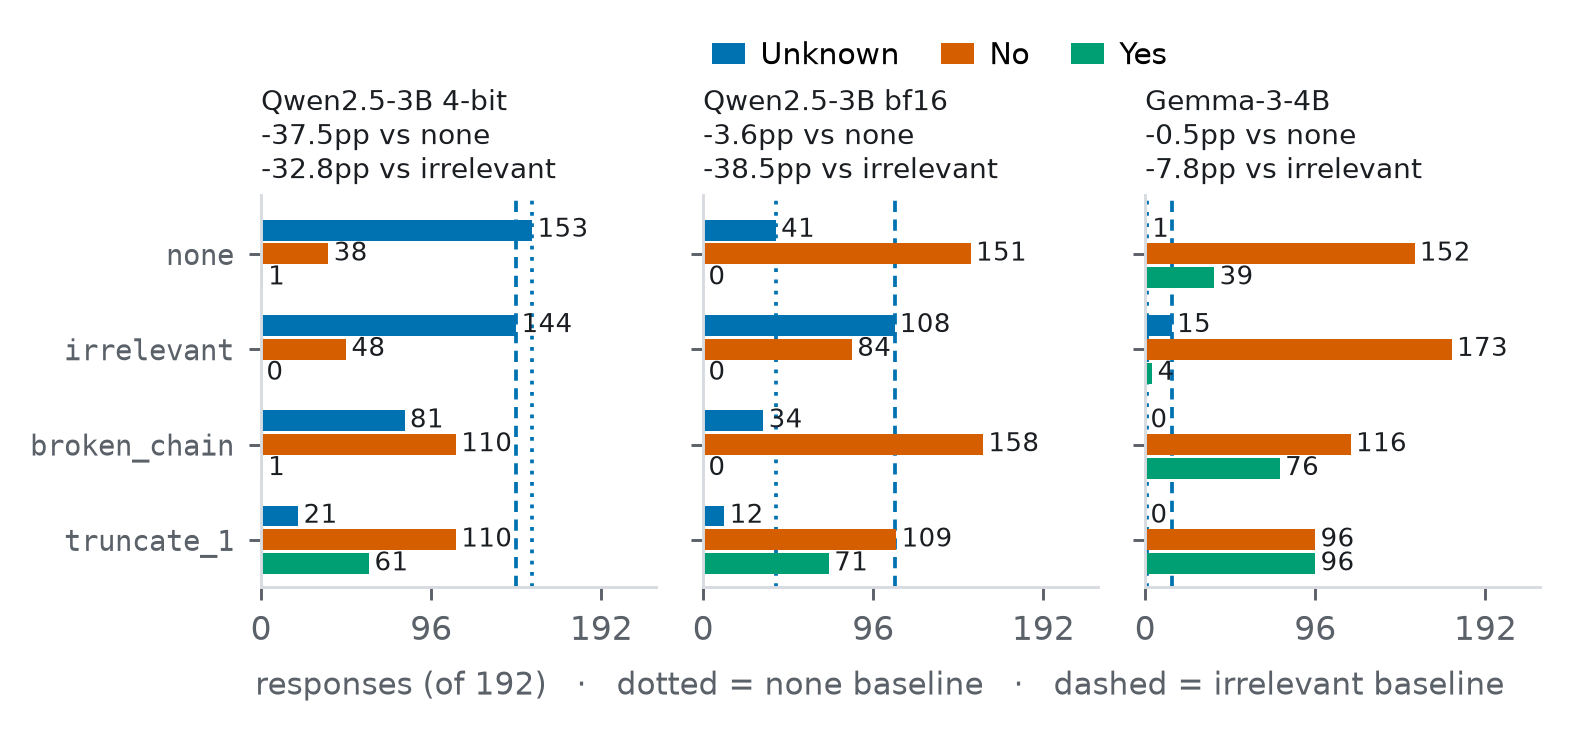
\includegraphics[width=1.0\textwidth]{figures/detection_response_distribution.png}
\caption{Three-candidate response distribution, three checkpoints, four arms.
Dotted and dashed lines mark the \textsc{none} and \textsc{irrelevant} abstention
baselines, $4.7$pp apart at 4-bit and $34.9$pp at bfloat16. A
broken chain lowers abstention against \emph{both} references on every checkpoint, the opposite of the
direction validity detection predicts.}
\label{fig:detection}
\end{figure}

\textbf{Reversing the final rule and the premise it fires on costs accuracy on
every checkpoint.} Separating them does not. The split is post hoc:
\textsc{shuffled} moves three things at once, so we re-scored the same items
under eight permutations each on all three checkpoints, recording where those
two lines landed. An identity arm reproduces \textsc{truncate\_1}'s bytes and
returns its receipts $192/192$ throughout. Distance is flat; direction is not
(\cref{fig:order}). Rule \emph{after} its premise gives $26.8$, $22.4$ and $94.9\%$ across the three checkpoints against
$5.8$, $4.8$ and $84.9\%$ for rule \emph{before}; paired within item on the
4-bit checkpoint, $45$ items favour rule-after against $2$
($p = 1.6\times10^{-11}$). The direction holds everywhere, its size does not: a
$4.6\times$ ratio on the Qwen checkpoints is a $10$pp modulation on Gemma-3-4B.

\textbf{Nothing defends against a wrong solver.} The \textsc{misleading} arm is
identical to \textsc{full} except in its last two sentences: a fabricated final
rule, absent from the theory, and the inverted literal it licenses. The
ground-truth answer is unchanged. All three checkpoints answer incorrectly on
\textbf{$189$, $186$ and $192$ of $192$} items, at $d'$ of $-4.36$, $-4.06$ and
$-5.13$: the model exploiting surface overlap most is also the one most
completely misled. The class split is sharper. Gemma-3-4B's standing prior is
\texttt{No} --- under \textsc{none} it answers \texttt{No} to all $192$ items,
at $c = 2.565$ --- and under \textsc{misleading} it answers \texttt{Yes} on $93$
of the $96$ contradicted items. A fabricated rule inverts a near-total prior.

\textbf{This does not attenuate with scale.} Llama-3.3-70B, sixteen times the
largest of the three above, scores $0$ of $192$ under \textsc{misleading} at
$d' = -5.12$, with no item within $0.5$ logits of the boundary. It is not
struggling: $192/192$ under \textsc{full}, $191/192$ under
\textsc{broken\_chain}, and $145$ of $192$ with no certificate at all. A single
fabricated rule inverts every one of them. Qwen3-32B is not interpretable here: it fails the
per-class recall floor under \textsc{full} at $0.167$ while clearing three other
arms, and the reason is measurement rather than the model --- the pair we score
disagrees with the token it would emit on $5$ of $12$ sampled items in that arm,
against $12/12$ where it is confident. We record it and draw nothing from it.

Whether any model notices, we cannot say. Rescoring \textsc{broken\_chain} with
an \texttt{Unknown} candidate available should raise abstention if the model
tracks validity. It falls by $37.5$ and $32.8$ points against \textsc{none} and
\textsc{irrelevant} and \emph{rises} by $31.2$ against the surface-matched
\textsc{truncate\_1}
(\cref{fig:detection}): the sign is a function of the reference, and neither
reference is clean. We draw no conclusion from it and withdraw the claim that it
refutes detection. What needs no reference is that the most capable of the three
abstains $0$ times in $192$ on a broken certificate and answers \texttt{Yes} on
$76$. No positive evidence, then, that any checkpoint verifies validity --- and
the corruption arm above is direct evidence that none does.

\section{Limitations}

\textbf{Scope of the mechanism claim.} On both Qwen checkpoints the inference is
exactly one step deep: withholding two steps scores identically to no
certificate ($0/96$). Gemma-3-4B is not in that position ($4/96$ against
$22/96$ unaided), so depth is checkpoint-specific, as is the share:
$40.4$--$98.6\%$ against the \textsc{irrelevant} control, $51.4$--$98.6\%$
against unaided. The full theory is visible in every arm, so breaking a
certificate is diagnostic only where the model scores $0/96$ from the theory
alone --- true of both Qwen checkpoints, not of Gemma-3-4B, where $20$ of its
$22$ unaided successes recur under \textsc{broken\_chain}. A model using a broken
certificate as a pointer back into the theory would be doing inference of a
different kind; we record that as an interpretation caveat, not a controlled
alternative. \textsc{truncate\_2} and \textsc{truncate\_3} also drop the query
predicate, confounding depth with predicate presence, and an undecidable
\textsc{proof\_prefix} cannot contain it either.

\textbf{Post hoc analyses and superseded criteria.} The $2\times2$ reading of
the reanalysis, the sweep's replacement viability criterion and the
gap-versus-direction split are all post hoc, labelled where used, with the
originals retained in the released results. The reanalysis carries five
defects we report rather than repair: a prespecified $15$pp target with only
$8.3$pp of headroom above the $91.7\%$ arm it applied to; no recorded proof
depth, so its failures cannot be stratified; task identifiers encoding the
semantic class; a flat receipt export with no sealed panel, so its answer key is
reconstructed from those identifiers; and a leak screen that was a malformed
regular expression and never fired (the released certificates contain none,
checked after the fact). Every later experiment fixes all five.

\textbf{Candidate tokenisation.} The prompt ends \texttt{Answer:}, inviting a
space-prefixed continuation, while the scored candidates are the bare tokens.
Only their relative order matters, and on the checkpoint carrying the scale
claim the two pairs agree on all $36$ sampled verdicts, diverging only near
indifference --- which is why Qwen3-32B is not interpreted.

\textbf{The scale check is one checkpoint.} Llama-3.3-70B extends the corruption
result past the small-model reading, but it is one model at that scale, scored
through a fourth backend, and its unaided competence leaves the validity share
undefined: the denominator of \cref{sec:broken} collapses once a checkpoint can
answer without the record. Its $191/192$ under \textsc{broken\_chain} is not
evidence of detection either --- the theory is visible in every arm, and a model
with that much unaided competence may simply be ignoring a useless record. What
the arm shows is narrower and harder to explain away: a fabricated rule
overrides reasoning the model demonstrably has.

\textbf{Generalisation.} One task family, small models plus one 70B scale check,
synthetic panels.
Invented vocabularies establish item novelty, not independence from every
relevant pretraining pattern \citep{golchin2023time,deng2024investigating};
model is not randomised, so cross-model comparisons are descriptive. The
abstention rescoring changes the instruction and candidate set, and response
distributions move substantially \citep{zhao2021calibrate,zheng2023large}, so
its contrasts hold and its absolute rates do not. The reanalysis and validity
control use a 4-bit checkpoint and the sweep bfloat16 --- different artefacts of
one model --- and the sweep also chose the validity control's checkpoints,
leaving Phi-4-mini unrun on those arms. Every response is a forced choice among
verified single-token candidates, as no deployed setup is. At $n = 96$ the
loglinear correction censors $d'$ at $\pm 5.13$, where eight cells of
\cref{tab:arms} sit, so differences involving a saturated arm are bounds. The
reanalysis's per-arm counts and primary contrast appeared in an earlier
unpublished report by the present authors, which concluded the 3B checkpoint
failed an open-world unknown gate the sweep finds the family clears; differing
panels, candidate sets and quantisation plausibly explain it, and we flag it
rather than leave a reader to find both. Finally, every theory here arrives
\emph{already formalised}: nothing tests whether a model can turn a prose
framework into solver input, which the corruption result makes consequential.

\section{Conclusion}

End-to-end accuracy cannot say why solver assistance helps. The decomposition
can: arrange the arms so each contrast moves one factor, and break validity
while holding surface form fixed. Applied across fourteen models, two inference
stacks and $38{,}424$ responses, it returns a different answer almost
every time it is asked --- a validity share of $98.3\%$ on one checkpoint and
$40.4$--$51.4\%$ on another, with depth, order-sensitivity and viability itself
properties of a checkpoint, an arm and a runtime. We offer the method and
decline to generalise its value, ours included.

One result does not move. Given a certificate whose fabricated final rule
establishes the negation, the three checkpoints answer incorrectly on $189$,
$186$ and $192$ of $192$, and none abstains; nor is it a small-model artefact,
since a $70.6$B checkpoint that solves $145$ of $192$ unaided is wrong on all
$192$. Mechanism claims about solver assistance do not transfer between
checkpoints; the failure to check the solver does. So run a corrupted arm,
report per checkpoint, and report sensitivity beside accuracy --- two criteria
we had prespecified were gamed by label collapse.

\section*{Reproducibility Statement}

\textbf{Code and data.} The supplementary material accompanying this submission
is self-contained: sealed panels and answer authorities, all $38{,}424$
per-response receipts, the generators, runners, audits and analysis scripts, and
the forward-closure certifier with its validation against the public corpus.
Every number in this paper can be re-derived from a fresh unpack with no network
access, no model weights and no external packages; the audits use the Python standard
library only, so verification does not depend on resolving an
environment. Panels are hash-stamped, and the runners for the validity control and the model sweep refuse a panel
whose hash does not match, while the others record the hash without enforcing it.
The answer authority is opened after all receipts are written, by convention in
the analysis order rather than by a gate in the code. Scoring takes the
highest-likelihood candidate token; on an exact tie the first candidate in the
declared order wins, which across the validity control's $5{,}760$ prospective responses
occurs twice. Each receipt carries a SHA-256 of its own contents,
and all $38{,}424$ verified with zero failures. The count is not typed into the manuscript: it is
produced by \texttt{scripts/census\_receipts\_v1.py} from the released receipts
and substituted at compose time.

\textbf{Checking one number takes a minute.} \texttt{scripts/verify.py} recomputes each headline value and prints it beside the
value this paper states. Nine of its eleven claims re-derive
from the receipts and the sealed panels; the cross-model mean and the model table
read released analysis files, which the listed scripts regenerate:
\texttt{python3 scripts/verify.py validity-share} recomputes the $98.3\%$ of
\cref{sec:broken} and shows the four counts it came from.
\texttt{--all} adds Gemma's two baselines, the corruption counts at both scales,
the detection direction on three checkpoints, the $2\times2$ state main effect,
the cross-model mean, the response census, a recomputed digest for every one of
the $38{,}424$ receipts, all sixty cells of \cref{tab:models}, and the
ten printed properties of the worked example in \cref{tab:stimulus}. It uses the
standard library only, so a reviewer needs no environment beyond Python. Model weights are not redistributed, but each run records the
pinned revision and a hash of the weight files before those files are deleted. A
permanent archive with a DOI will accompany the camera-ready version.

\section*{AI-Use Statement}

A large language model was used as a coding and drafting assistant throughout:
generating experiment code, analysis scripts and figure code, and drafting this
manuscript. All experimental design decisions, the interpretation of results,
and the claim boundaries were made and verified by the authors. Every numeric
value reported was produced by the released analysis scripts from sealed
receipts, not written by a model; the released audits allow any reader to
re-derive them independently.

\bibliographystyle{iclr2027_conference}
\bibliography{refs}

\end{document}
